\documentclass{article}%
\usepackage{tikz}
\usetikzlibrary{arrows}
\usepackage{amsmath}%
\usepackage{amsfonts}%
\usepackage{amssymb}%
\usepackage{graphicx}
\usepackage[]{algorithm2e}
%-------------------------------------------
\newtheorem{theorem}{Theorem}
\newtheorem{acknowledgement}[theorem]{Acknowledgement}
%\newtheorem{algorithm}[theorem]{Algorithm}
\newtheorem{axiom}[theorem]{Axiom}
\newtheorem{case}[theorem]{Case}
\newtheorem{claim}[theorem]{Claim}
\newtheorem{conclusion}[theorem]{Conclusion}
\newtheorem{condition}[theorem]{Condition}
\newtheorem{conjecture}[theorem]{Conjecture}
\newtheorem{corollary}[theorem]{Corollary}
\newtheorem{criterion}[theorem]{Criterion}
\newtheorem{definition}[theorem]{Definition}
\newtheorem{example}[theorem]{Example}
\newtheorem{exercise}[theorem]{Exercise}
\newtheorem{lemma}[theorem]{Lemma}
\newtheorem{notation}[theorem]{Notation}
\newtheorem{problem}[theorem]{Problem}
\newtheorem{proposition}[theorem]{Proposition}
\newtheorem{remark}[theorem]{Remark}
\newtheorem{solution}[theorem]{Solution}
\newtheorem{summary}[theorem]{Summary}
\newenvironment{proof}[1][Proof]{\textbf{#1.} }{\ \rule{0.5em}{0.5em}}
\setlength{\textwidth}{7.0in}
\setlength{\oddsidemargin}{-0.35in}
\setlength{\topmargin}{-0.5in}
\setlength{\textheight}{9.0in}
\setlength{\parindent}{0.3in}
\linespread{1.55}
\begin{document}

\begin{flushright}
\textbf{Brandon Toner \\
\today}
\end{flushright}

\begin{center}
\textbf{CSCI 405: Algorithm Analysis II \\
Homework 4: Depth-First Search} \\
\end{center}



\begin{enumerate}
\item  DVS-Comp and DFS-VISIT-Comp \\
\begin{algorithm}[H] 
 \TitleOfAlgo{DFS-Comp}
 \KwData{$G$}
 \ForEach{Vertex $\mu \in G.V$} {
   $\mu.color = WHITE$\;
   $\mu.\pi = NULL$\;
 }
 $time = 0$\;
 $c = 1$ \;
 \ForEach{Vertex $\mu \in G.V$} {
   \If { $\mu.color == WHITE$} {
     DFS-VISIT-Comp(G, $\mu$, c)\;
     $c = c + 1$\;
   }
 }
\end{algorithm}

\begin{algorithm}[H]
 \TitleOfAlgo{DFS-VISIT-Comp}
 \KwData{$G, \mu, c$}
 $time = time + 1$\;
 $\mu.d = time$\;
 $\mu.color = GRAY$\;
 $\mu.c = c$\;
 \ForEach{Vertex $v \in G.Adj[\mu]$} {
   \If {$v.color == WHITE$} {
     $v.\pi = \mu$\;
     DFS-VISIT-Comp($G, v, c$)\;
   }
 }
 $\mu.color = BLACK$\;
 $time = time + 1$\;
 $\mu.f = time$\;
\end{algorithm}
\item If we start at node $\alpha$, in whose adjacency list $\mu$ comes before $v$, $\mu$ will finish before $v$ is discovered, but there is a path from $\mu$ to $v$. \\
\begin{tikzpicture}[->,>=stealth',shorten >=1pt,auto,node distance=3cm,
  thick,main node/.style={circle,fill=blue!20,draw,font=\sffamily\Large\bfseries}]

  \node[main node] (1) {$\alpha$};
  \node[main node] (2) [below left of=1] {$\mu$};
  \node[main node] (4) [below right of=1] {$v$};

  \path[every node/.style={font=\sffamily\small}]
    (1) edge node [left] {} (4)
        edge [bend right] node[left] {} (2)
    (2) edge [bend right] node [right] {} (1);
\end{tikzpicture}


\item Using the same graph and adjacency lists as in (2), we find that $\mu$ is discovered before $v$, but $v$ is not $G_{\pi}$ descendant of $\mu$.
\end{enumerate}
\end{document}
